\documentclass{article}
\usepackage[utf8]{inputenc}
\usepackage{listings}
\usepackage{multimedia} % to embed movies in the PDF file
\usepackage{graphicx}
\usepackage{comment}
\usepackage[english]{babel}
\usepackage{amsmath}
\usepackage{amsfonts}
\usepackage{subfigure}
\usepackage{wrapfig}
\usepackage{multirow}
\usepackage{verbatim}
\usepackage{float}

\newtheorem{theorem}{Theorem}[section]
\newtheorem{lemma}[theorem]{Lemma}
\newtheorem{corollary}[theorem]{Corollary}
%\newtheorem{algorithm}[theorem]{Algorithm}
\newtheorem{remark}[theorem]{Remark}
\newenvironment{proof}{\noindent {\bf Proof:} }{\hfill $\Box$ \\[2ex] }
\newenvironment{keywords}{\begin{quote} {\bf Key words} }
                         {\end{quote} }
\newenvironment{AMS}{\begin{quote} {\bf AMS subject classifications} }
                         {\end{quote} }


\newcommand{\eref}[1]{\mbox{\rm(\ref{#1})}}
\newcommand{\tref}[1]{\mbox{\rm\ref{#1}}}
\newcommand{\set}[2]{\left\{ #1 \; : \; #2 \right\} }
\newcommand{\deq}{\raisebox{0pt}[1ex][0pt]{$\stackrel{\scriptscriptstyle{\rm def}}{{}={}}$}}

\newcommand {\DS} {\displaystyle}

\newcommand{\real}{\mathbb{R}}
\newcommand{\compl}{\mathbb{C}}



\newcommand {\half} {\mbox{$\frac{1}{2}$}}
\newcommand{\force}{{\mathbf{f}}}
\newcommand{\strain}{{\boldsymbol{\varepsilon}}}
\newcommand{\stress}{{\boldsymbol{\sigma}}}
\renewcommand{\div}{{\boldsymbol{\nabla}}}

\newcommand {\cA} {{\cal A}}
\newcommand {\cB} {{\cal B}}
\newcommand {\cC} {{\cal C}}
\newcommand {\cD} {{\cal D}}
\newcommand {\cE} {{\cal E}}
\newcommand {\cL} {{\cal L}}
\newcommand {\cP} {{\cal P}}
\newcommand {\cQ} {{\cal Q}}
\newcommand {\cR} {{\cal R}}
\newcommand {\cV} {{\cal V}}
\newcommand {\cW} {{\cal W}}
\newcommand {\CH} {{\cal H}}
\newcommand {\CS} {{\cal S}}


\newcommand{\bzero}{\mathbf{0}}
\newcommand{\ba}{\mathbf{a}}
\newcommand{\bb}{\mathbf{b}}
\newcommand{\bc}{\mathbf{c}}
\newcommand{\bd}{\mathbf{d}}
\newcommand{\be}{\mathbf{e}}
\newcommand{\bff}{\mathbf{f}}
\newcommand{\bg}{\mathbf{g}}
\newcommand{\bh}{\mathbf{h}}
\newcommand{\bn}{\mathbf{n}}
\newcommand{\bp}{\mathbf{p}}
\newcommand{\bq}{\mathbf{q}}
\newcommand{\br}{\mathbf{r}}
\newcommand{\bs}{\mathbf{s}}
\newcommand{\bt}{\mathbf{t}}
\newcommand{\bu}{\mathbf{u}}
\newcommand{\bv}{\mathbf{v}}
\newcommand{\bw}{\mathbf{w}}
\newcommand{\bx}{\mathbf{x}}
\newcommand{\by}{\mathbf{y}}
\newcommand{\bz}{\mathbf{z}}
\newcommand{\bA}{\mathbf{A}}
\newcommand{\bB}{\mathbf{B}}
\newcommand{\bC}{\mathbf{C}}
\newcommand{\bD}{\mathbf{D}}
\newcommand{\bE}{\mathbf{E}}
\newcommand{\bF}{\mathbf{F}}
\newcommand{\bG}{\mathbf{G}}
\newcommand{\bH}{\mathbf{H}}
\newcommand{\bI}{\mathbf{I}}
\newcommand{\bJ}{\mathbf{J}}
\newcommand{\bK}{\mathbf{K}}
\newcommand{\bL}{\mathbf{L}}
\newcommand{\bM}{\mathbf{M}}
\newcommand{\bN}{\mathbf{N}}
\newcommand{\bO}{\mathbf{O}}
\newcommand{\bP}{\mathbf{P}}
\newcommand{\bQ}{\mathbf{Q}}
\newcommand{\bR}{\mathbf{R}}
\newcommand{\bS}{\mathbf{S}}
\newcommand{\bU}{\mathbf{U}}
\newcommand{\bV}{\mathbf{V}}
\newcommand{\bW}{\mathbf{W}}
\newcommand{\bX}{\mathbf{X}}
\newcommand{\bY}{\mathbf{Y}}
\newcommand{\bZ}{\mathbf{Z}}

\newcommand{\cO}{ {\cal O} }
\newcommand{\CT}{ {\cal T} }
\newcommand{\IL}{{\mathbb L}}
\newcommand{\sIL}{{{{\mathbb L}_s}}}
\newcommand{\bOmega}{{\boldsymbol{\Omega}}}
\newcommand{\bPsi}{{\boldsymbol{\Psi}}}

\newcommand{\bgamma}{{\boldsymbol{\gamma}}}
\newcommand{\bmu}{{\boldsymbol{\mu}}}
\newcommand{\blambda}{{\boldsymbol{\lambda}}}
\newcommand{\bLambda}{{\boldsymbol{\Lambda}}}
\newcommand{\bpi}{{\boldsymbol{\pi}}}
\newcommand{\bPi}{{\boldsymbol{\Pi}}}
\newcommand{\bphi}{{\boldsymbol{\phi}}}
\newcommand{\bPhi}{{\boldsymbol{\Phi}}}
\newcommand{\bpsi}{{\boldsymbol{\psi}}}
\newcommand{\btheta}{{\boldsymbol{\theta}}}
\newcommand{\bTheta}{{\boldsymbol{\Theta}}}
\newcommand{\bSigma}{{\boldsymbol{\Sigma}}}
\newcommand{\sump}{\sideset{}{^{'}}\sum} 
\DeclareMathOperator*{\Res}{Res}
\DeclareMathOperator{\OO}{O}
\DeclareMathOperator{\oo}{o}
\DeclareMathOperator{\erfc}{erfc}
\def\Xint#1{\mathchoice
   {\XXint\displaystyle\textstyle{#1}}%
   {\XXint\textstyle\scriptstyle{#1}}%
   {\XXint\scriptstyle\scriptscriptstyle{#1}}%
   {\XXint\scriptscriptstyle\scriptscriptstyle{#1}}%
   \!\int}
\def\XXint#1#2#3{{\setbox0=\hbox{$#1{#2#3}{\int}$}
     \vcenter{\hbox{$#2#3$}}\kern-.5\wd0}}
\def\ddashint{\Xint=}
\def\pvint{\Xint-}






\title{AMATH 585 Homework 3}
\author{Cade Ballew}
\date{January 31, 2022}

\begin{document}
	
	\maketitle
	
	\section{Problem 1}
	\subsection{Part a}
Considering an initial guess of
\[
\theta(t)=0.7+t(t-2\pi)^2
\]
with a stepsize of $h=1/80$, we are able to produce yet another solution to the nonlinear problem in the text different from those illustrated in figures 2.4 and 2.5 which is displayed in the following plot. \\
	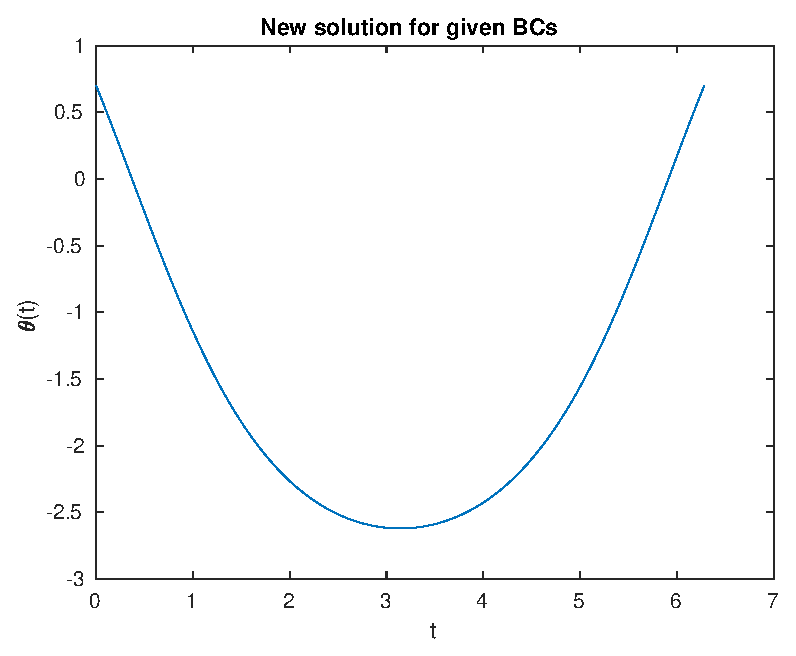
\includegraphics[scale=0.8]{hw3p1a.eps}\\

	\subsection{Part b}
To find a solution to this BVP with the same general behavior as figure 2.5 for a longer time interval, we choose our initial guess based on properties at our initial time interval $T=2\pi$. Namely, we reuse the computed solution for a smaller $T$ by using it as an initial guess (after scaling to the new time interval appropriately) for a larger time interval. The following plots display the solution that we obtain for $T=20,50,100,200$ by doing this recursively. \\
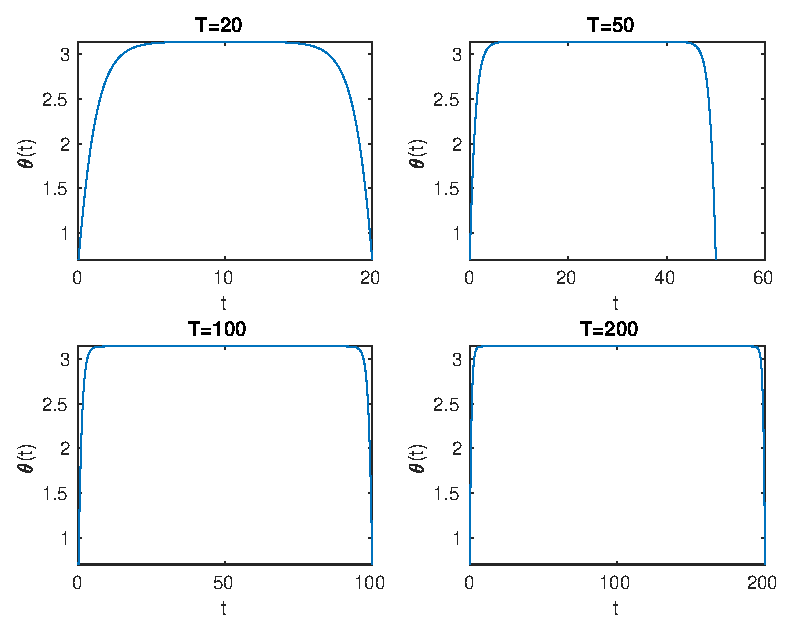
\includegraphics{hw3p1b.eps}\\
The following table lists the maximum value of $\theta$ obtained in each time interval. Clearly, they appear to be converging to $\pi$.
\begin{table}[H]\centering
\begin{tabular}{|r|r|}\hline
{T}&{$\max_i\theta_i$}\\\hline
$2\pi$&2.8975061095462498\\
20&      3.1413385828458429\\
50&      3.1415926535120287\\
100&      3.1415926535897931\\
200&     3.1415926535897931\\\hline
\end{tabular}
\end{table}
The following MATLAB code was used the obtain the results for this problem. 
\begin{verbatim}
clear

T=2*pi;
m=2001;
t=linspace(0,T,m+2)';
h = t(2)-t(1);
alpha=0.7; beta=0.7;

theta=0.7+t.*(t-2*pi).^2;


theta = theta(2:end-1); %remove boundary
tol=1e-12; itermax=1000;
[theta,~,~]=NewtonSolve(theta,alpha,beta,h,tol,itermax);
figure(1)
plot(t,theta)
plot(t,theta)
xlabel('t'); ylabel('\theta(t)')
title('New solution for given BCs')
saveas(gcf,'hw3p1a','epsc')

i=1;
fprintf('T           max(theta)\n')

theta=0.7+sin(t/2);
theta = theta(2:end-1); %remove boundary
[theta,~,~]=NewtonSolve(theta,alpha,beta,h,tol,itermax);
fprintf('%i      %16.16d\n',T,max(theta))
figure(2)
for T=[20,50,100,200]
t=linspace(0,T,m+2)';
h = t(2)-t(1);
theta = theta(2:end-1); %remove boundary, reuse old theta as new guess
[theta,~,~]=NewtonSolve(theta,alpha,beta,h,tol,itermax);
subplot(2,2,i)
plot(t,theta)
title(['T=',num2str(T)])
xlabel('t')
ylabel('\theta(t)')
fprintf('%i      %16.16d\n',T,max(theta))
i=i+1;   
end
saveas(gcf,'hw3p1b','epsc')

function G=buildG(theta,alpha,beta,h)

G=zeros(length(theta),1);
theta = [alpha; theta; beta]; %include BCs for computation 
for i=1:length(theta)-2
G(i)=(theta(i)-2*theta(i+1)+theta(i+2))/h^2+sin(theta(i+1));
end

end


function J=buildJ(theta,h)

maindiag=-2+cos(theta)*h^2;
J=spdiags([ones(length(theta),1),maindiag,ones(length(theta),1)],-1:1,...
length(theta),length(theta));
J=J/h^2;

end


function [theta,iter,dnormvec]=NewtonSolve(initial_guess,alpha,beta,h,tol,itermax)

theta = initial_guess;
deltanorm=Inf;
iter=0;
while deltanorm>tol && iter<itermax
G=buildG(theta,alpha,beta,h);
J=buildJ(theta,h);
delta=-J\G;
theta=theta+delta;
deltanorm=norm(delta,'inf');
iter=iter+1;
dnormvec(iter)=deltanorm;
end

theta=[alpha;theta;beta]; %add BCs

end
\end{verbatim}
	
	\section{Problem 2}
	\subsection{Part a}
%add equations once you have internet
By Gerschgorin's theorem, we can sum the absolute values of the non-diagonal entries of the coefficient matrix $A$ associated with this set of difference equations to get that the Gerschgorin disks are given by
\[
B\left(\frac{2}{h^2}+1+x_1^2,\frac{1}{h^2}\right)=B\left(\frac{2}{h^2}+1+h^2,\frac{1}{h^2}\right)
\]
for $i=1$,
\[
B\left(\frac{2}{h^2}+1+x_m^2,\frac{1}{h^2}\right)=B\left(\frac{2}{h^2}+1+h^2m^2,\frac{1}{h^2}\right)
\]
for $i=m$, and
\[
B\left(\frac{2}{h^2}+1+x_i^2,\frac{2}{h^2}\right)=B\left(\frac{2}{h^2}+1+h^2i^2,\frac{2}{h^2}\right)
\]
for $i=2,\ldots,m-1$. We know that the eigenvalues of $A$ must be contained in the union of these disks, so observing that $A$ is symmetric so all eigenvalues are real, 
\begin{align*}
&\min_{i\in\{2,\ldots,m-1\}}\left\{\frac{1}{h^2}+1+h^2,\frac{1}{h^2}+1+h^2m^2,1+h^2i^2\right\}\leq\lambda\\&\leq\max_{i\in\{2,\ldots,m-1\}}\left\{\frac{3}{h^2}+1+h^2,\frac{3}{h^2}+1+h^2m^2,\frac{4}{h^2}+1+h^2i^2\right\}
\end{align*}
if $\lambda$ is an eigenvalue of $A$. Making the assumption that $m\geq1$ so that $0<h\leq\frac{1}{2}$, we can easily reduce this to 
\[
\min\left\{\frac{1}{h^2}+1+h^2,1+h^22^2\right\}\leq\lambda\leq\max\left\{\frac{3}{h^2}+1+h^2m^2,\frac{4}{h^2}+1+h^2(m-1)^2\right\}.
\]
Now, we note that with our restrictions on $m$ and $h$, $3h^4\leq3(1/2)^4=3/8<1$, so $1+4h^2<\frac{1}{h^2}+1+h^2$. Similarly, we can also conclude that $\frac{3}{h^2}+1+h^2m^2<\frac{4}{h^2}+1+h^2(m-1)^2$, so we can bound the eigenvalues of $A$ by
\[
1+4h^2\leq\lambda\leq\frac{4}{h^2}+1+h^2(m-1)^2.
\]
	\subsection{Part b}
To see that the $L_2$-norm of the global error is the same order as the local truncation error, we borrow the book's notation and use the inequalities on page 19 to write
\[
\|E\|_{L_2}\leq\|A^{-1}\|_{L_2}\|\tau\|_2=\left(\min_i|\lambda_i|\right)^{-1}\|\tau\|\leq\|\tau\|=\OO(h^2).
\]
The reason for this is that we know that 1 is a lower bound on the eigenvalues of $A$, because the lower bound we found in part a is clearly greater than 1 when $h>0$.
	
	\section{Problem 3}

	\section{Problem 4}

\end{document}
